\subsection{Quo Vadis, Action Recognition? A New Model and the Kinetics Dataset}

\subsubsection{Overview}
This paper by Carreira \textit{et al} introduces a new model for the task of action recognition, called \textit{Two-Stream Inflated 3D ConvNet (I3D)}. It involves a discussion on the following:
\begin{itemize}
\item A comparison between 2D kernels and 3D kernels
\item Using optical flow along with RGB input
\item How information is propagated through time (frames) when using 2D convolutional networks.
\item Whether transfer learning, i.e., training on one dataset for some task and then applying the pre-trained network on another task by optional fine-tuning, has benefits for video tasks
\end{itemize}

\subsubsection{Datasets}
The paper compares the performance of all models on the task of action recognition using the following datasets:
\begin{itemize}
\item Pre-training on the Kinetics Human Action Video Dataset \cite{kay2017kinetics}
\item Fine-tuning on HMDB-51 \cite{kuehne112011hmdb}
\item Fine-tuning on UCF-101 \cite{soomro2012ucf101}
\end{itemize}

\subsubsection{Compared Models}
The paper compares the models shown in Figure \ref{fig:carreira2018quo-models}.

\begin{figure}

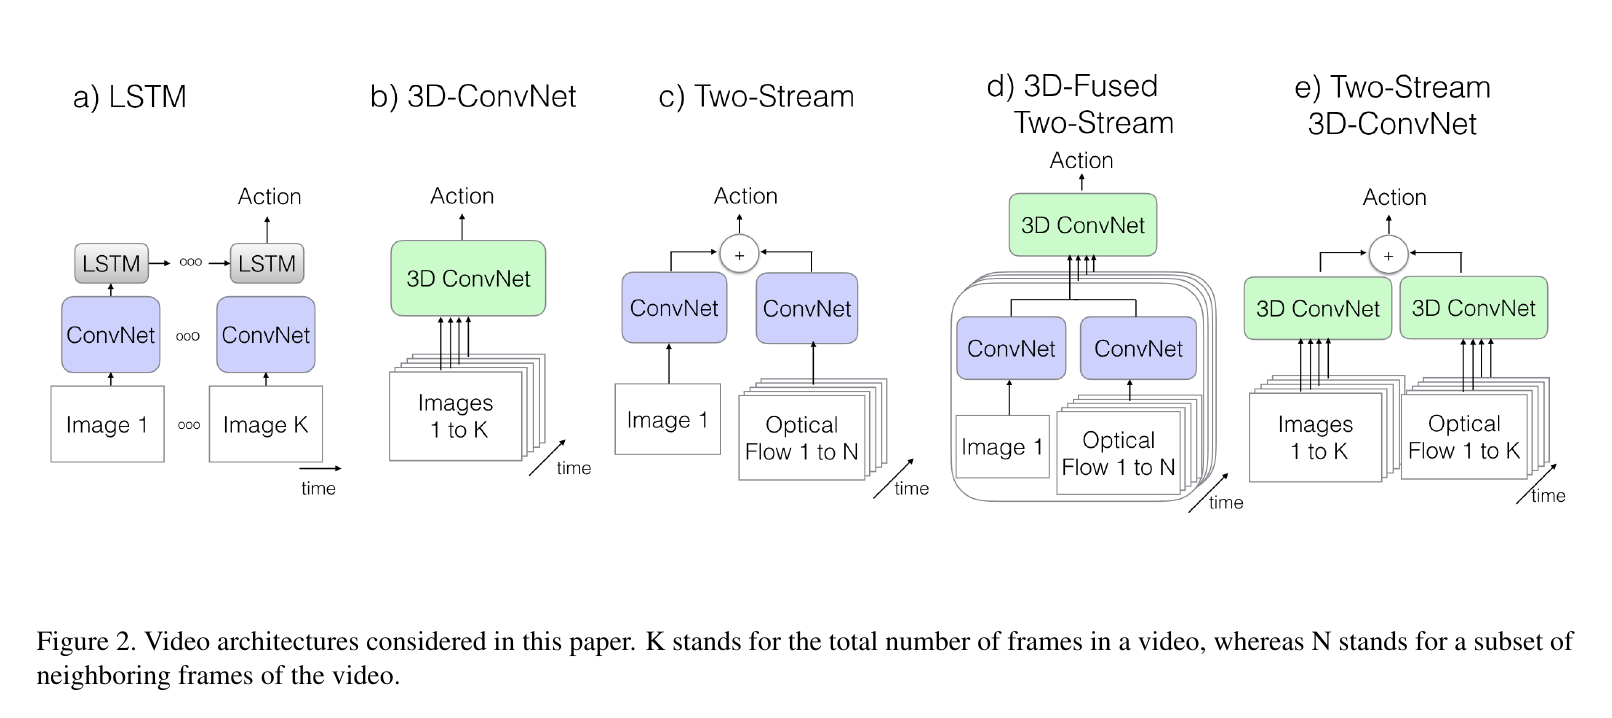
\includegraphics[width=\linewidth]{assets/img/carreira2018quo-models.png}
\caption{The models compared by Carreira \textit{et al}. Image Courtesy \cite{carreira2018quo}}
\label{fig:carreira2018quo-models}

\end{figure}

\paragraph{ConvNet + LSTM}
Using successful image classification networks only, features are extracted from each frame 
of the video and predictions are (independently) pooled across the whole video. This 
architecture completely ignores the temporal structure of the video, i.e. notions of 
before-after, forward-backward in time are not learned.

\paragraph{3D ConvNet}
Instead of standard 2D ConvNets, this model uses convolutional networks with 
\textit{spatio-temporal} filters. They are able to directly create hierarchical 
representations of spatio-temporal data (videos in this case). But because of an additional 
kernel dimension, (1) They have many more parameters than 2D ConvNets, making them much 
harder to train and (2) We also cannot make use of pre-trained networks (e.g. on ImageNet). 
Due to these reasons, previous work with 3D ConvNets are mostly involve shallow 
architectures, trained from scratch.

\paragraph{Two-Stream Networks}
Capturing low-level motion using LSTMs after last layers of convolutional networks is very 
expensive to train as it requires unrolling the network through multiple frames. In this 
architecture, short temporal snapshots are modelled by averaging predictions from a single 
RGB frame and 10 optical flow frames, after these two streams are passed through identical 
ConvNets (pre-trained on ImageNet). Multiple such snapshots are sampled from the video and 
action prediction is averaged. This architecture is very efficient to train and test. An 
extension to this involves fusing spatial and optical flow streams after the last 
convolutional layer.

\paragraph{Two-Stream Inflated 3D ConvNets (I3D)}
Carreira \textit{et al} introduce this novel model for the action recognition task 
\cite{carreira2018quo}. Following characteristics explain the working of this model:

\subparagraph{Inflating 2D ConvNets into 3D} The trick this architecture employs is to 
simply convert 2D ConvNets (successful ones, pre-trained on ImageNet) into 3D ConvNets. This 
conversion is done by inflating filters and pooling kernels, i.e. adding a temporal 
dimension to them. Hence filters go from 2D to 3D.

\subparagraph{Bootstrapping 3D filters from 2D filters}
The parameters from successful ImageNet models can be used directly in the I3D ConvNet. This 
is done by repeating the weights of the 2D filters $N$ times along the time dimension, and 
rescaling them by dividing by $N$. This implicitly pre-trains the 3D model on ImageNet. The 
authors call this the \textit{boring-video fixed point} \cite{carreira2018quo}.

\subparagraph{Receptive Field}
In image models, symmetric receptive fields, say $F \times F$, are not optimal when 
considering the time dimension, since the frame rate should also be considered. If the field 
grows too quickly in time relative to space, edges from different objects might get 
combined, which would lead to poor features in the initial part of the model. If it grows 
too slowly, the scene dynamics might not be captured well. The \textit{boring-video fixed 
point} allows freedom on choosing how to inflate pooling operators along the time dimension 
and on choosing the temporal stride \cite{carreira2018quo}.

\subparagraph{Two 3D Streams}
A 3D ConvNet can learn features just from RGB input, but using optical flow too is found to 
be helpful. This is because with RGB input, pure feedforward computation is performed, but 
optical flow algorithms have some recurrence. Hence, similar to Two-Stream networks, a 
two-stream configuration is used - one I3D network for RGB, one for optical flow. The two 
networks are trained separately and their predictions are averaged.

\subsubsection{Performance}
Carreira \textit{et al} compare their I3D model (with only RGB, only optical flow and both 
streams) with other types of models, with and without pre-training on datasets such as 
ImageNet and Kinetics. The models are evaluated on HMDB-51 and UCF-101, and their 
Two-Stream I3D, pre-trained on ImageNet and Kinetics outperforms all models on these 
datasets in terms of classification accuracy for action recognition. 

\subsubsection{Conclusion}
The authors claim that based on these results, it is evident that there is a considerable 
benefit in pre-training on Kinetics for the action recognition task 
\cite{carreira2018quo}. Moreover, the results indicate that using 3D kernels is better for 
video tasks than using 2D kernels, and using optical flow along with RGB input has 
benefits, since it adds recurrence.